\documentclass[12pt]{article}
\usepackage[utf8]{inputenc}
\usepackage{sbc-template}
\usepackage{graphicx,url}
\usepackage{import}
\usepackage[brazilian]{babel}
\usepackage[latin1]{inputenc}  

     
\sloppy

\title{Microcontrolador PIC18F452\\Organização e Arquitetura}

\author{Eduardo José dos Reis Nobre Junior\inst{1}}


\address{Universidade Estadual de Santa Cruz
  (UESC)\\
  Caixa Postal 45662-900 Campus Soane Nazaré de Andrade, \\Rodovia Jorge Amado, Km 16, Bairro Salobrinho, Ilhéus-Bahia 
}

\begin{document} 

\maketitle

\begin{abstract}
	The PIC18F452 Microcontroller used in monitoring activities of equipment, instrumentation and monitoring, data acquisition. Using the RISC architecture, equipped with internal memory divided into instruction memory and data memory. Capable of parallel communication and simultaneous access to data and instructions by using Harvard architecture, thus having separate buses for memory and instructions. This article aims to present the characteristics from the point of view of its organization and architecture and how certain characteristics can be used by the user.
\end{abstract}
     
\begin{resumo} 
	O Microcontrolador PIC18F452 utilizado em atividades de monitoramento de equipamento, instrumentação e monitoramento, aquisição de dados. Utilizando a arquitetura RISC, dotado de memória interna dividida em em memória de instrução e memória de dados. Capaz de comunicação paralela e acesso simultâneo a dados e instruções por utilizar a arquitetura Harvard, tendo portanto barramentos separados para memória e instruções.  Esse artigo visa apresentar as características a partir do ponto de vista da sua organização e arquitetura e como certas características podem ser utilizadas pelo usuário.
\end{resumo}


\section{Visão Geral e Organização}
O Microcontrolador PIC18F452 utilizado em atividades de monitoramento de equipamento, instrumentação e monitoramento, aquisição de dados. Utilizando a arquitetura RISC, dotado de memória interna dividida em em memória de instrução e memória de dados.
Capaz de comunicação paralela e acesso simultâneo a dados e instruções por utilizar a arquitetura Harvard.
\section{Organização de memória} 
A memória é dividida em três grupos descritos abaixo
\begin{itemize}
	\item Memória de Programa
	\item RAM de Dados
	\item EEPROM de Dados
\end{itemize}
\subsection{Memória de Programa}
Um Program Counter de 21 bits é capaz de endereçar o espaço de memória de 2 MB. Acessar um espaço entre a memória física e a memória de 2 MB causará a leitura de todos zeros, uma instrução NOP.\\
O tendo 32 KBytes de memória Flash,  podendo armazenar palavras de instruções de 16K.
O endereço  do vetor de RESET é encontrado em 00000H e os vetores de interrupções se encontram nos endereços 00008h e 00018h.
\begin{figure}[ht]
\centering
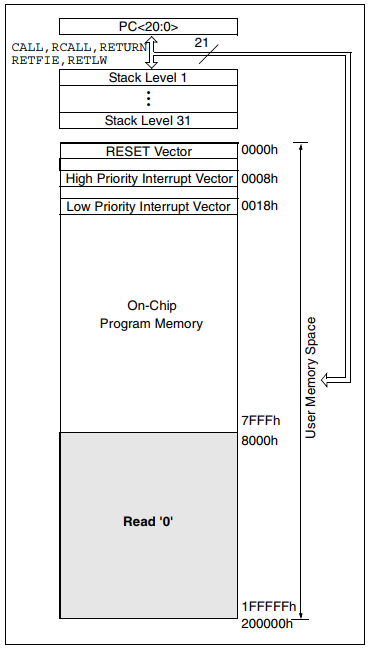
\includegraphics[width=.5\textwidth]{figs/memory-1.png}
\caption{Figura 1. Mapa de Memória e Pilha, \texit{Fonte: \cite{knuth:84}}}
\end{figure}
\subsection{Instruções na Memória Programa}
A memória de instruções é acessada em bytes. Instruções são armazenadas como 2 ou 4 bytes na memória. O Least Significant Byte (LSB) de uma palavra de instrução sempre é armazenado num local de memória de endereço pár (LBS=’0’).\\
As instruções CALL e GOTO possuem um endereço absoluto de memória na instrução. Instruções são sempre armazenadas no espaço de uma palavra, os dados contidos em uma instrução são um endereço.
\subsection{Organização da Memória de Dados}
A memória de dados é implementada com o uso de SRAM. Cada registro na memória de dados tem um endereço de 12 bits, permitindo o armazenamento de até 4096 bytes. O mapa de memória é dividido em 16 bancos contendo 256 bytes cada. O últimos 4 bits do Bank Select Register (BSR) selecionam qual banco será acessado. Os primeiros 4 bits do BSR não são implementados. A memória de dados contém Special Function Registers (SFR) e General Purpose Registers (GPR) Os SFR são utilizados para controle, status do controlador e funções auxiliares, enquanto GPR são utilizados para armazenamento de dados.
\\\\Toda memória pode ser acessada diretamente ou indiretamente. Acesso direto talvez necessite do uso de um registrador BSR. Acesso indireto necessita do uso de um File Select Register (FSRn) e um correspondente Indirect (INDFn). Cada FSR armazena endereços de 12 bits que podem ser utilizados para acessar qualquer valor do mapa de da memória de dados.
\\\\O conjunto de instruções e arquitetura permite operações entre todos os bancos. Isso pode se realizado por endereçamento indireto com o uso da instrução MPVFF. 
\subsection{Memória de Programa Flash}
A memória de instruções Flash suporta operações de leitura e escrita. Uma leitura na memória de instrução é executada um byte por vez. Uma escrita realizada na memória de instrução é executada em blocos de 8 bytes por vez.
\\Escrever ou apagar a memória de instruções irá interromper operações de buscas até que a operação seja realizada. A memória não pode ser acessada durante a escrita ou remoção de instruções, portanto, codígo não pode ser executado.
\subsection{Memória de dados EEPROM}
A memória de dados EEPROM suporta operações de leitura e escrita durante a operação normal. A memória de dados não é diretamente mapeada no espaço de do registrado, é registrado portanto por Special Function Registers.
\\Existem quatro SFR utilizados para leitura e escrita de programas e dados na memória EEPROM. Esses registrados são EECON1 EECON2 EEDATA EEADR.
\subsection{Pilha de retorno de endereço}
A pilha de retorno de endereço permite até 31 chamadas de instruções e interrupções em qualquer combinação. O PC é colocado no topo da pilha quando as instruções CALL ou RCALL  são executadas ou uma interrupção é reconhecida, armazenando o endereço anterior para posterior utilização usando as instruções RETURN, RETLW ou RETFIE para pegar o valor de PC da pilha.
\\A pilha opera com uma estrutura de 31 palavras de 21 bits na RAM e uma pilha de ponteiros de 5 bits, com a pilha de ponteiros inicializada com 00000b após todos os RESETS. Não há RAM associada com o pilha de ponteiros 00000b.
\\O espaço de pilha não faz parte nem da memória de instruções nem de dados. A pilha de ponteiro aceita operações de leitura e escrita, o topo da pilha pode ser acessado através de registradores SFR. Dados podem ser colocados e removidos do topo da pilha utilizando operações SFR. Um bit de sinal indica se o ponteiro da pilha se encontra acima ou no limite de 31 fornecidos.
\subsection{Fluxo de dados e Pipeline}
Um ciclo de instruções consiste em quatro Q ciclos (Q1, Q2, Q3, Q4). A instrução de busca e execução passam pelo pipeline de forma que a operação de busca dure um ciclo de instrução enquanto a decodificação e execução da instrução duram outro ciclo. Se uma instrução fizer com que o PC se altere, dois ciclos serão necessários para a conclusão da instrução.
\\Um ciclo de busca começando com o PC sendo incrementado para Q1.No ciclo de instrução, a instrução buscada é levada ao IR no ciclo Q1. Essa instrução então é decodificada e executada nos ciclos seguintes. Dados são lidos durante Q2 e escritos em Q4, na leitura do operando e escrita do destino.
\begin{figure}[ht]
	\centering
	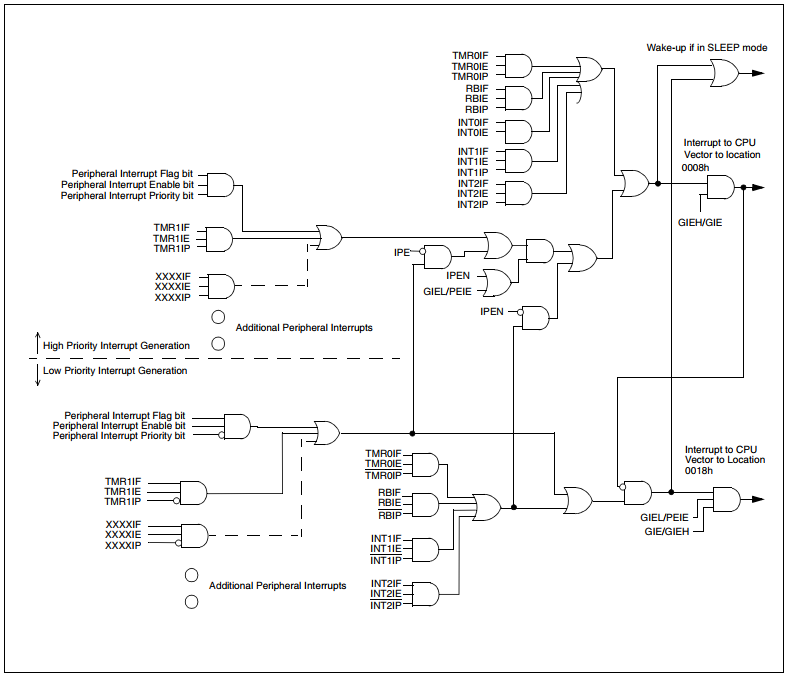
\includegraphics[width=.5\textwidth]{figs/interrupt.png}
	\caption{Figura 2. Estrutura do sistema de interrupções, \texit{Fonte: \cite{knuth:84}}}
\end{figure}
\section{Interrupções}
O microcontrolador possui múltiplas fontes de interrupção e uma característica que permite cada fonte de interrupção ser associada a um nível de prioridade. O vetor de interrupções de alta prioridade se encontra no endereço 000008h e o vetor de interrupções de baixa prioridade se encontra no endereço 000018h. Interrupções de alta prioridade sobrescreveram interrupções que esteja em andamento. O dispositivo possui 10 registradores responsáveis por controlar as operações de interrupção.
\begin{itemize}
	\item RCON
	\item INTCON
	\item INTCON2
	\item INTCON3
	\item PIR1, PIR2
	\item PIE1, PIE2
	\item IPR1, IPR2 
\end{itemize}
Cada fonte de interrupção, exceto INT0, possui três bits para controlar suas operações. Esses bits são:
\begin{itemize}
	\item Bit de flag para indicar que um evento de interrupção ocorreu. 
	\item Bit de enable que permite que o programa em execução se desvie quando esse bit está acionado. 
	\item Bit de prioridade configurado para high ou low. 
\end{itemize}
Quando uma interrupção é respondida, o Global Interrupt Enable (GIE) é limpo para desabilitar futuras interrupções. Se o bit de prioridade estiver limpo esse se torna o bit de GIE. Se níveis de prioridade forem utilizados, estes serão os bits GIEH ou GIEL.
\\O endereço de retorno é colocado na pilha de endereços citadas na sessão X o PC é carregado com o endereço do vetor de instruções (000008h ou 000018h). Uma vez que no Interrupt Service Routine, a fonte da interrupção pode ser determinada ao se ler os bits flags da interrupção. Os bits de interrupção devem ser limpos antes do religamento do sistema de interrupções para evitar interrupções recursivas.
\section{Entrada e Saida}
Dependendo do modelo do dispositivo, existem cinco ou três portas disponíveis. Alguns dos pinos de I/O são multiplexados com uma função alternativa.
\\Cada porta tem três registradores para essa operação, sendo eles:
\begin{itemize}
	\item TRIS 
	\item PORT 
	\item LAT 
\end{itemize}
Os registradores acima são separados em 5 grupos A, B, C, D e E criando TRIS\textsubscript{A}, TRIS\textsubscript{B} e assim por diante.
\begin{table}[h]
	\centering
	\caption{Tabelas de Características do Registrador PORT}
	\begin{tabular}{llllll}
		\hline
		PORT & A & B & C & D & E\\
		\hline
		Largura & 7 bits & 8 bits & 8 bits & 8 bits & 3 bits\\
		\hline
		Bi-directional & Sim & Sim & Sim & Sim & Sim 
	\end{tabular}
\end{table}

Cada registrador PORT possui um conjunto de pinos R\textsubscript{A}, R\textsubscript{B}… Esses pinos podem ser utilizados para leitura ou gravação, analógica ou digital.
\\O registrador TRIS\textsubscript{A} controla a direção dos pinos R\textsubscript{A}, mesmo quando eles estão sendo utilizados de forma analógica, trocando os pinos de entrada para saída.
\\O usuário deve garantir que os bits no registrador TRIS\textsubscript{A} estejam configurados quando utilizando RA como entrada analógica.
\\O registrado LAT\textsubscript{A} está mapeado na memória. Operações de leitura e escrita em LAT\textsubscript{A} escreve os valores como entrada ou saída em PORT\textsubscript{A}. Essa situação se mantém verdadeira para LAT\textsubscript{E} e PORT\textsubscript{E}, LAT\textsubscript{C} e PORT\textsubscript{C} e por seguinte.
\section{Conjunto de Instruções}
\\O PIC18 possui um conjunto de instruções que melhora a versão anterior PICmicro, mantendo ainda a fácil migração do conjunto de instruções do PICmicro.
\\A maioria das instruções são palavras únicas de 16 bits, mas existem três instruções que requerem dois espaços de instrução.
\\Cada palavra é dividida em um OPCODE, que especifica o tipo da instrução e um ou mais operandos. O conjunto de instruções é extremamente ortogonal e é agrupado nas categorias abaixo:
\begin{itemize}
	\item Instruções orientadas a Byte 
	\item Instruções orientadas a Bit 
	\item Instruções Literais 
	\item Instruções de Controle
\end{itemize}
\clearpage
\\A maioria das instruções \textbf{orientadas a Byte} contem três operandos:
\begin{enumerate}
	\item O registrador de arquivo \textbf{(f)}
	\item O destino do resultado \textbf{(d)}
	\item A memóra acessada \textbf{(a)}
\end{enumerate}
\\O registrador de arquivo f especifica qual registrador de arquivo deverá ser utilizado pela instrução.
\\O destino do resultado d específica onde o resultado da operação será colocado. Se o d tem o valor de 0, o resultado devera ser colocado no registrador WREG. Se o valor de d for 1, o resultado deverá ser colocado no registrador especificado na instrução.

\\A maioria das instruções \textbf{orientadas a Bit} contem três operandos:
\begin{enumerate}
	\item O registrador de arquivo \textbf{(f)}
	\item O bit do registrador de arquivo \textbf{(b)}
	\item A memóra acessada \textbf{(a)}
\end{enumerate}
\\O bit do registrador de arquivo b seleciona o número do bito afetado pela operação, enquanto o designador do registrador de arquivo f representa o número do arquivo no qual o bit está localizado.
\begin{figure}[h]
	\centering
	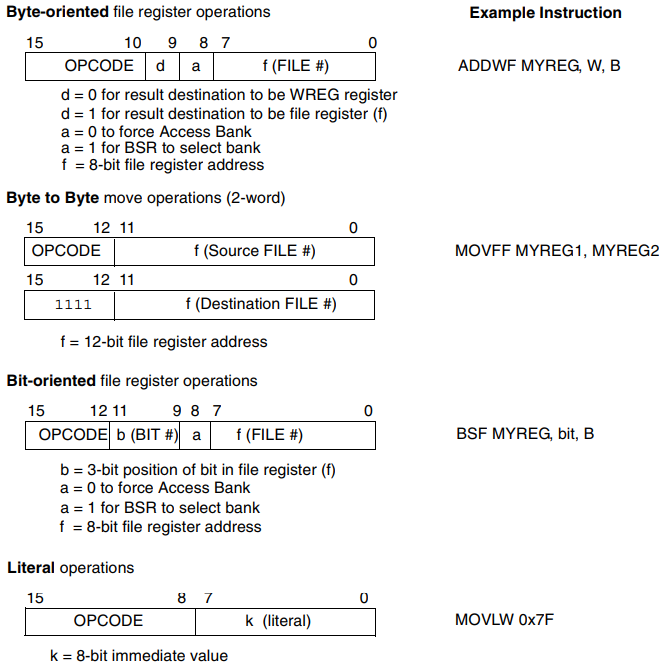
\includegraphics[width=.5\textwidth]{figs/instructions.png}
	\caption{Figura 3. Estrutura geral das Instruções, \texit{Fonte: \cite{knuth:84}}}
\end{figure}
\clearpage
\\Instruções \textbf{literais} podem usar os seguintes operandos:
\begin{enumerate}
	\item Um valor literal a ser carregado em um registrador de arquivo \textbf{(k)}
	\item O registrador FSR a ser carregado o valor do literal \textbf{(f)}
	\item Operando não requerido \textbf{(--)}
\end{enumerate}
\\Instruções de \textbf{controle} podem usar os seguintes operandos:
\begin{enumerate}
	\item Um endereço de memória de programa \textbf{(n)}
	\item O modo das instruções de Call e Return \textbf{(s)}
	\item O modo das instruções Table Read e Table Write \textbf{(s)}
	\item Operando não requerido \textbf{(--)}
\end{enumerate}
\begin{figure}[h]
	\centering
	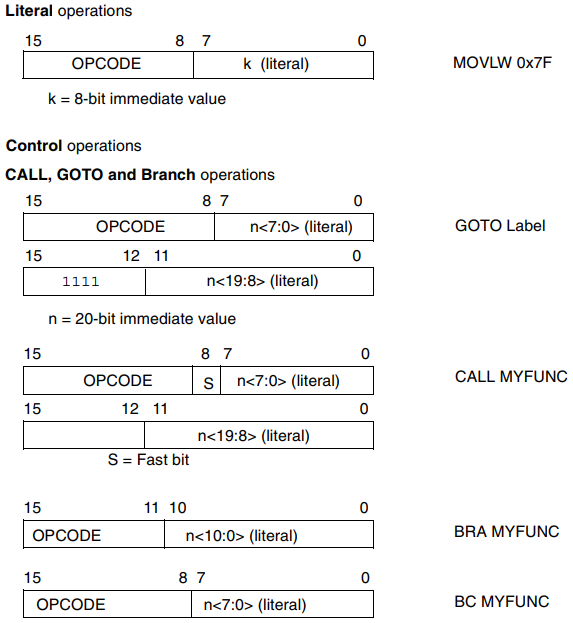
\includegraphics[width=.5\textwidth]{figs/instructions-2.png}
	\caption{Figura 3. Estrutura geral das Instruções, \texit{Fonte: \cite{knuth:84}}}
\end{figure}
\clearpage
\bibliographystyle{sbc}
\bibliography{sbc-template}

\end{document}
